% Domain-Augmented LLMs for Scientific Visualization
\documentclass{vgtc}                          % final (conference style)

\ifpdf%
  \pdfoutput=1\relax
  \pdfcompresslevel=9
  \pdfoptionpdfminorversion=7
  \ExecuteOptions{pdftex}
  \usepackage{graphicx}
  \DeclareGraphicsExtensions{.pdf,.png,.jpg,.jpeg}
\else%
  \ExecuteOptions{dvips}
  \usepackage{graphicx}
  \DeclareGraphicsExtensions{.eps}
\fi%

\graphicspath{{figures/}{pictures/}{images/}{./}}

\usepackage{microtype}
\PassOptionsToPackage{warn}{textcomp}
\usepackage{textcomp}
\usepackage{mathptmx}
\usepackage{times}
\renewcommand*\ttdefault{txtt}
\usepackage{cite}
\usepackage{booktabs}
\usepackage{listings}
\usepackage{xcolor}

\onlineid{0}
\vgtccategory{Research}
\vgtcinsertpkg

\title{Domain-Grounded Tool Orchestration for LLM-Guided Scientific Analysis}

\author{Jeff Lee\thanks{e-mail: jeff.lee@kitware.com}\\ %
        \scriptsize Kitware, Inc. %
\and Sebastien Jourdain\thanks{e-mail: sebastien.jourdain@kitware.com}\\ %
     \scriptsize Kitware, Inc. %
\and Corey Quammen\thanks{e-mail: corey.quammen@kitware.com}\\ %
     \scriptsize Kitware, Inc. %
\and Patrick O'Leary\thanks{e-mail: patrick.oleary@kitware.com}\\ %
     \scriptsize Kitware, Inc. %
\and Berk Geveci\thanks{e-mail: berk.geveci@kitware.com}\\ %
     \scriptsize Kitware, Inc.}

\abstract{%
Scientific analysis workflows encode deep domain knowledge through sequences
of tightly coupled operations where correctness depends on tool selection,
execution order, and parameterization.
A CFD engineer investigating flow separation must extract wall shear stress,
identify zero-crossings in skin friction, and confirm with boundary layer
profiles---a chain that requires both domain expertise and proficiency with
visualization tools.
Current approaches to LLM-assisted scientific visualization generate scripts
that encode this knowledge implicitly and often incorrectly---producing code
that executes but yields wrong results.
We present an architecture that separates intent interpretation (LLM) from
execution (deterministic domain tools) from explanation (LLM), connected by
the Model Context Protocol (MCP) and grounded by domain ontologies that
constrain planning to valid analysis chains.
We demonstrate the approach in two domains on the same ParaView server
infrastructure: computational fluid dynamics post-processing and topological
data analysis via the Topology ToolKit (TTK).
Adding the second domain required only an ontology and tool wrappers around
existing filters---no changes to the architecture, protocol, or deployment.
Evaluated on canonical analysis scenarios in both domains, the approach
produces physically and topologically correct results where script generation
produces silent failures, and scales to production datasets via ParaView's
client-server architecture.%
}

\CCScatlist{
  \CCScat{I.3.6}{Computer Graphics}{Methodology and Techniques}{Interaction techniques};
  \CCScat{I.6.6}{Simulation and Modeling}{Simulation Output Analysis}{}
}

\begin{document}

\firstsection{Introduction}

\maketitle

Scientific toolkits for data analysis and visualization are remarkably capable.
ParaView~\cite{Ahrens:2005:PEO} provides hundreds of filters for processing
simulation data.
The Topology ToolKit (TTK)~\cite{Tierny:2018:TTK} offers persistence diagrams,
Morse-Smale complexes, contour trees, and critical point extraction.
3D Slicer~\cite{Fedorov:2012:3DS} contains hundreds of modules for medical
image analysis.
The computational capability exists.
The gap is not in the tools but in their accessibility: given a scientific
question, which tools should be applied, in what order, with what parameters,
and what do the results mean?

Large language models (LLMs) offer a natural interface for bridging this gap.
A user can state an engineering question---``is there flow separation on the
upper surface?''---and an LLM can, in principle, translate that into the
appropriate sequence of analysis operations.
However, current approaches to LLM-assisted scientific visualization conflate
two fundamentally different tasks: deciding \textit{what} to analyze (an intent
interpretation problem where LLMs excel) and \textit{how} to execute the
analysis (a procedural domain knowledge problem where deterministic tools are
superior).

The dominant paradigm---LLM-generated scripts---asks the model to produce
executable code that directly invokes visualization APIs.
Recent work by Zhao et al.~\cite{Zhao:2026:RAG} demonstrates that even with
retrieval-augmented generation (RAG), this approach suffers from API
hallucination, missing pipeline stages, and wrong-strategy errors.
Their error taxonomy reveals that the hardest failures are not syntactic but
strategic: the LLM chooses the wrong analysis approach entirely, producing code
that executes but answers the wrong question.
These are domain knowledge failures, not code quality failures, and they cannot
be resolved by better code generation.

We propose an architecture that assigns each task to the component best suited
for it.
The LLM interprets user intent and explains results---tasks that require natural
language understanding and synthesis.
Deterministic domain tools execute the analysis---tasks that require validated,
reproducible procedures.
The Model Context Protocol (MCP)~\cite{MCP:2024} provides a standardized
interface between them.
A domain ontology constrains the LLM's planning to physically or topologically
valid analysis chains, preventing the wrong-strategy errors that persist in
script generation approaches.

We demonstrate that this pattern generalizes across scientific domains by
implementing it for two distinct applications on the same ParaView server
infrastructure: computational fluid dynamics (CFD) post-processing and
topological data analysis via TTK.
Both domains exhibit the same structural challenge---powerful tools that
require expert knowledge to configure, chain, and interpret---and both
benefit from the same architectural solution.
Adding the second domain required only an ontology file and MCP tool wrappers
around existing TTK filters; no changes to the architecture, protocol,
deployment, or user interface.

Our contributions are:
\begin{enumerate}
\item A \textbf{Plan--Execute--Interpret} architecture with domain ontology
and MCP tool layer that separates intent interpretation from execution from
explanation.
\item \textbf{CFD instantiation} with three use cases demonstrating diagnostic
reasoning: validated analysis from natural language, iterative multi-step
investigation, and cross-quantity synthesis.
\item \textbf{TTK instantiation} with three use cases: topological feature
identification, structural decomposition, and comparative topology across
timesteps.
\item Evidence that both domains \textbf{compose on the same server instance},
and that the marginal cost of adding a domain is an ontology and tool wrappers.
\item Demonstration that \textbf{tool orchestration produces correct results}
where script generation produces silent failures.
\item \textbf{Scalable deployment} via ParaView's client-server architecture
with a thin browser client.
\end{enumerate}


\section{Related Work}

\textbf{LLM-assisted visualization code generation.}
Several systems have explored using LLMs to generate visualization code.
ChatVis~\cite{Chen:2024:ChatVis} presents an iterative assistant that generates
Python scripts for data analysis and visualization, relying on chain-of-thought
prompting and execution feedback for correction.
VisGene~\cite{Li:2025:VisGene} proposes a multi-agent framework for scientific
visualization in HPC environments, integrating LLM-generated VTK/Python modules
with retrieval-augmented generation and fine-tuned vision models.
Most recently, Zhao et al.~\cite{Zhao:2026:RAG} investigate structure-aware RAG
for vtk.js pipeline generation, curating a corpus of code examples with
module-level metadata and using module overlap rather than semantic similarity
for retrieval.
These approaches share a common architecture: the LLM generates executable code
that directly invokes visualization APIs.
The limitations are structural.
Generated scripts are one-shot---no structured results flow back for the LLM to
reason about.
Correction is human-driven, not system-driven.
And the most dangerous failure mode---code that executes but performs the wrong
analysis---is not addressed by better code generation.

\textbf{Natural language interfaces for scientific tools.}
Natural language interfaces for visualization have been explored extensively in
the chart-oriented domain~\cite{Luo:2022:NL2VIS,Li:2024:MatPlotAgent}, where the
mapping from intent to visual encoding is relatively direct.
Scientific visualization presents a harder problem: the mapping from an
engineering question to a multi-step analysis procedure requires domain
expertise that varies across disciplines, solvers, and data formats.
No existing system maps natural language to physically validated, multi-step
CFD or topological analysis chains.

\textbf{Tool use and agentic architectures.}
The Model Context Protocol (MCP)~\cite{MCP:2024} standardizes how LLMs discover
and invoke external tools, providing typed parameters, structured return values,
and a stateless protocol over stateful backends.
Function calling and tool use in LLMs have been explored through
ReAct~\cite{Yao:2023:ReAct} and chain-of-thought
prompting~\cite{Wei:2022:CoT}.
Our work differs in that the tools return structured quantitative data---not
confirmation messages or rendered images---enabling the LLM to perform
quantitative reasoning in the interpretation phase.

\textbf{Domain ontologies in scientific computing.}
Ontologies for scientific simulation have been developed across
CFD, structural mechanics, and materials science.
Knowledge graphs have been applied to scientific workflow management and
data provenance.
Our contribution is an ontology specifically designed to ground LLM planning
in domain knowledge, mapping observable phenomena to the physical quantities
that reveal them and the analysis tools that extract those quantities.


\section{Architecture}
\label{sec:arch}

This section presents the domain-independent architectural pattern.
\autoref{sec:cfd} and \autoref{sec:ttk} instantiate it for CFD and
topological data analysis.

\subsection{System Overview}

The system comprises four layers (\autoref{fig:architecture}):
(1)~a \textbf{browser client} that receives compressed rendered frames and
sends user input---no data or geometry reaches the browser, as rendering is
performed entirely server-side via ParaView's \texttt{VtkRemoteView};
(2)~a \textbf{trame web server}~\cite{Jourdain:2023:trame} that mediates
between the browser and the ParaView backend, hosting the LLM integration
and MCP tool dispatch;
(3)~an \textbf{LLM with domain ontology} that interprets user intent, plans
analysis operations constrained by the ontology, and interprets structured
results returned by tools;
(4)~a \textbf{ParaView server} (\texttt{pvserver}) that holds all data,
executes the visualization pipeline, and renders frames, optionally running
MPI-parallel on a compute node with both CFD filters and TTK filters
available as ParaView plugins.

The same codebase runs in two modes: in-process via \texttt{pvpython} for
development, or client-server via \texttt{pvserver} for production.
A dual-mode data access helper transparently selects between in-process access
and client-server fetch based on the active connection type.

\begin{figure}[tb]
 \centering
 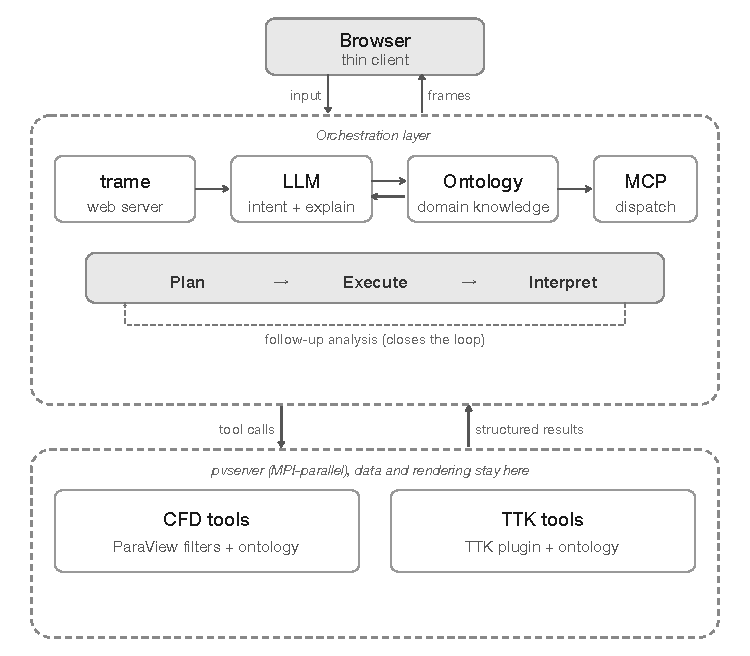
\includegraphics[width=\columnwidth]{figures/architecture}
 \caption{System architecture. The browser is a thin client receiving only
 rendered frames. The LLM plans analysis operations constrained by the domain
 ontology, dispatches them via MCP to deterministic tools running on
 \texttt{pvserver}, and interprets the structured results. Both CFD and TTK
 tools execute on the same server instance. The Plan--Execute--Interpret loop
 closes when the Interpret phase proposes follow-up analysis.}
 \label{fig:architecture}
\end{figure}

\subsection{The Plan--Execute--Interpret Loop}

Each user interaction initiates a cycle through three phases.

\textbf{Plan (Intent Resolution).}
The user states a question in domain language.
The LLM consults the domain ontology, which maps observable phenomena to the
physical quantities that indicate them and the tools that extract those
quantities.
The ontology \textit{constrains} the plan: rather than choosing freely from
all possible ParaView operations, the LLM selects from the subset that the
ontology declares valid for the identified phenomenon.
The output is an ordered sequence of named tool invocations with parameters.

\textbf{Execute.}
MCP dispatches the planned tool calls to the ParaView pipeline.
Tools are deterministic domain workflows---not generated scripts---that build
or modify the server-side pipeline and return structured results: field
statistics, extracted profiles, integrated quantities, topological invariants.
Critically, tools return \textit{data}, not \textit{renders}.
The pipeline persists across invocations, enabling multi-step analysis within
a single session.

\textbf{Interpret.}
The LLM receives the structured results along with the relevant ontology entry.
It generates a grounded explanation with quantitative specifics (``separation
detected at $x/c = 0.72$ based on $C_f$ sign reversal'') rather than generic
commentary.
The ontology's \texttt{follow\_ups} field provides diagnostic reasoning chains:
if separation is detected, the ontology recommends confirming with boundary
layer profiles and checking for upstream transition.
When the interpretation identifies a finding that warrants further investigation,
it proposes a follow-up analysis, closing the loop back to the Plan phase.

\subsection{Domain Ontology}

The ontology follows a domain-independent schema with five fields per entry:
\textit{phenomenon} (an observable feature or condition),
\textit{indicators} (quantities that reveal it),
\textit{tools} (operations that extract those quantities),
\textit{follow-ups} (what to investigate next),
and \textit{significance} (why it matters in the application context).
The same schema is instantiated with different content for each domain.
The CFD ontology contains approximately 30 entries covering external aerodynamics;
the TTK ontology contains approximately 25 entries covering topological features.
Each is authored by a domain expert in JSON and loaded at startup.

\autoref{fig:ontology} shows representative entries from the CFD and TTK
ontologies.
The ontology is deliberately small---capturing the high-leverage knowledge that
distinguishes expert analysis from naive tool application---rather than
attempting encyclopedic domain coverage.

\begin{figure}[tb]
\centering
\begin{lstlisting}[basicstyle=\scriptsize\ttfamily,frame=single,
  caption={Representative ontology entries.},label={fig:ontology},
  captionpos=b,abovecaptionskip=5pt]
// CFD ontology entry
{ "phenomenon": "flow_separation",
  "indicators": ["Cf_zero_crossing",
    "reversed_BL_velocity"],
  "tools": ["show_forces", 
    "show_boundary_layer"],
  "follow_ups": ["boundary_layer_profiles",
    "upstream_transition_check"],
  "significance": "Increases pressure drag,
    reduces lift, may indicate stall onset"
}

// TTK ontology entry
{ "phenomenon": "noisy_scalar_field",
  "indicators": ["many_low_persistence_pairs",
    "no_clear_persistence_gap"],
  "tools": ["compute_persistence",
    "persistence_curve", "simplify_field"],
  "follow_ups": ["re_extract_critical_points",
    "segment_morse_smale"],
  "significance": "Noise obscures real 
    structure; simplification required 
    before meaningful analysis"
}
\end{lstlisting}
\end{figure}

\subsection{MCP Tool Layer}

Tools are organized in two tiers.
\textbf{Domain workflow tools} encode expert knowledge about multi-step
analysis procedures.
In CFD, \texttt{show\_boundary\_layer} extracts a velocity profile normal to
the surface at a specified station and computes displacement thickness,
momentum thickness, and shape factor.
In TTK, \texttt{compute\_persistence} runs the persistence diagram filter and
returns birth-death pairs with types and persistence values.
These tools encapsulate the procedural knowledge that script generation handles
unreliably.
\textbf{Refinement tools} provide low-level control: changing color maps,
adjusting thresholds, modifying representation types.
These are domain-independent and shared across both instantiations.

Three design principles govern tool implementation.
\textit{Structured returns:} every tool returns quantitative data, not just
confirmation---data the interpretation phase can reason about.
\textit{Dynamic field resolution:} tools accept semantic field names
(``velocity,'' ``pressure'') and resolve them to solver-specific array names
at runtime using pattern matching and alias tables.
\textit{Safe pipeline management:} consumer-aware deletion prevents breaking
downstream filter dependencies, and infrastructure filters are automatically
reused when a matching instance already exists.

\subsection{Client-Server Deployment}

ParaView's client-server architecture provides scalability without
architectural changes.
The \texttt{pvserver} process runs on a compute node, holds all data in server
memory, executes the full visualization pipeline, and renders frames using
server-side GPUs.
The trame web server connects via \texttt{simple.Connect()} and forwards all
pipeline operations through ParaView's client-server protocol.
The browser receives only compressed JPEG frames---it never sees geometry or
field data.
Client memory remains constant regardless of dataset size; a 100-million-cell
mesh resides entirely on the server.
For analysis operations requiring local computation, a \texttt{fetch\_data}
helper transfers only extracted results (surfaces, profiles, integrated
quantities).


\section{Domain 1: Computational Fluid Dynamics}
\label{sec:cfd}

\subsection{Implementation}

The CFD instantiation wraps ParaView's visualization filters as MCP tools with
aerodynamics domain knowledge.
The ontology covers external aerodynamics phenomena including flow separation,
stagnation, recirculation, vortex breakdown, shock waves, and wake structure.
Each phenomenon maps to indicator quantities ($C_f$, $C_p$, wall shear stress,
velocity gradients, Q-criterion, total pressure loss) and the tools that
extract them.
The tool set includes
\texttt{show\_vortices} (Q-criterion or $\lambda_2$ isosurfaces),
\texttt{show\_streamlines} (seeded by wake extent detection),
\texttt{show\_boundary\_layer} (line probes normal to surface with integral
thickness computation),
\texttt{show\_forces} (pressure and viscous force integration with lift/drag
decomposition),
\texttt{show\_slice} (planar cuts with automatic field selection),
and \texttt{show\_flow\_topology} (vortex core line extraction).
Evaluation uses FUN3D and OpenFOAM datasets for external aerodynamics
configurations including airfoils, wings, and bluff bodies.

\subsection{Use Case: Natural Language to Validated Analysis}

A user asks: ``Is there flow separation on the upper surface?''

In the \textbf{Plan} phase, the LLM consults the CFD ontology.
The entry for ``separation'' identifies $C_f$ zero-crossing and reversed
velocity in the boundary layer as indicators, and maps these to
\texttt{show\_forces} (for skin friction extraction) and
\texttt{show\_boundary\_layer} (for velocity profile inspection).
The planner produces a two-step analysis chain: (1)~extract skin friction
coefficient on the upper surface, (2)~locate zero-crossings.

In the \textbf{Execute} phase, the tools run deterministically.
The surface is extracted, the skin friction field is resolved dynamically
(mapping ``skin friction'' to \texttt{Cf} in FUN3D, \texttt{wallShearStress}
in OpenFOAM), and zero-crossings are identified programmatically.
The tool returns structured data: a list of $x/c$ locations where $C_f$
changes sign, along with the $C_f$ distribution as an array.

In the \textbf{Interpret} phase, the LLM receives this structured data and the
ontology's significance entry for separation.
It produces: ``Separation detected at $x/c = 0.72$ on the upper surface based
on $C_f$ sign reversal.
Reattachment occurs at $x/c = 0.85$.
Recommend boundary layer profiles upstream and downstream to characterize the
separation bubble structure.''
The follow-up recommendation comes from the ontology's \texttt{follow\_ups}
field, not from the LLM's training alone.

\begin{figure*}[tb]
 \centering
 %% TODO: Use case walkthrough figure showing:
 %% Left: user query in chat UI
 %% Center: Plan (tool sequence), Execute (ParaView pipeline screenshot),
 %% Right: Interpret (structured output + explanation)
 %% Show the Cf distribution with zero-crossing marked
 \fbox{\parbox{0.95\textwidth}{\centering\vspace{1.5cm}
 \textbf{TODO: Use case walkthrough --- Natural Language to Validated Analysis}\\
 Left: chat UI with user query. Center: $C_f$ distribution with zero-crossing marked.\\
 Right: structured interpretation with follow-up recommendation.\\
 Show the Plan--Execute--Interpret cycle concretely.\vspace{1.5cm}}}
 \caption{Walkthrough of the validated analysis use case. The user asks
 about flow separation; the planner consults the ontology to select
 $C_f$ extraction; the tool returns structured data including zero-crossing
 locations; the interpreter produces a quantitative explanation with a
 physically motivated follow-up recommendation.}
 \label{fig:usecase_cfd}
\end{figure*}

\subsection{Use Case: Iterative Diagnostic Reasoning}

This use case demonstrates the closed-loop nature of the architecture.

\textbf{Step 1.} The user asks: ``Show me the pressure distribution.''
The planner maps this to surface $C_p$ extraction and color-mapped display.
After execution, the interpreter examines the $C_p$ distribution and identifies
a plateau on the upper surface between $x/c = 0.55$ and $x/c = 0.70$.
The ontology links $C_p$ plateaus to likely laminar separation bubbles
and recommends boundary layer profiles upstream and downstream.
The system reports: ``$C_p$ plateau detected on the upper surface between
$x/c = 0.55$--$0.70$, consistent with a laminar separation bubble.
Recommend boundary layer profiles at $x/c = 0.50, 0.60, 0.70, 0.80$.''

\textbf{Step 2.} The user approves the follow-up.
The planner invokes \texttt{show\_boundary\_layer} at four stations.
Each call returns a velocity profile array, displacement thickness $\delta^*$,
momentum thickness $\theta$, and shape factor $H$.
The interpreter synthesizes: ``Reverse flow detected at $x/c = 0.60$ and $0.70$,
confirming laminar separation.
Shape factor $H$ peaks at 4.2 at $x/c = 0.65$.
Attached profile recovered by $x/c = 0.75$ ($H = 1.8$), confirming turbulent
reattachment.
Separation bubble extends from $x/c \approx 0.57$ to $x/c \approx 0.73$.''

This multi-step diagnostic chain mirrors expert CFD practice.
Script generation cannot support it: scripts are one-shot, with no mechanism
for structured results to drive subsequent analysis.

\subsection{Use Case: Cross-Quantity Synthesis}

A user asks: ``What is driving the drag increase between $4^\circ$ and
$8^\circ$ angle of attack?''

The ontology's entry for drag identifies three components: pressure drag (from
$C_p$ integration), viscous drag (from wall shear integration), and wake
momentum deficit.
The planner decomposes the question:
(1)~compute pressure and viscous drag components for both angles via
\texttt{show\_forces},
(2)~extract separation location for both cases,
(3)~compare wake momentum deficit profiles.
All extractions execute within a persistent pipeline session---both datasets
remain loaded, and tools operate on each in turn.

The interpreter synthesizes: ``Separation moved forward from $x/c = 0.78$ at
$4^\circ$ to $x/c = 0.62$ at $8^\circ$.
Pressure drag increased 40\% while viscous drag remained roughly constant.
Wake momentum deficit increased 55\%.
Conclusion: separation-induced pressure drag dominates the drag increase,
consistent with incipient stall.''
No single tool call answers this question; the value is in orchestrated
multi-step reasoning where the ontology tells the planner how drag decomposes.


\section{Domain 2: Topological Data Analysis (TTK)}
\label{sec:ttk}

\subsection{Implementation}

TTK is a ParaView plugin---it runs on the same \texttt{pvserver} instance as
the CFD filters with no additional infrastructure.
Adding topological analysis required authoring a TTK-specific ontology and
implementing MCP tool wrappers around existing TTK filters.
The ontology covers topological phenomena including noise versus signal
features, dominant scalar field structures, merge/split events in contour
trees, and topological transitions under parameter variation.
Indicator quantities include persistence values, critical point counts and
types, Betti numbers, and Morse-Smale cell counts.

The tool set includes
\texttt{compute\_persistence} (persistence diagram with birth-death pairs),
\texttt{persistence\_curve} (feature count as a function of threshold),
\texttt{simplify\_field} (topological simplification below a persistence
threshold),
\texttt{critical\_points} (critical point extraction with type
classification),
\texttt{segment\_morse\_smale} (Morse-Smale complex with ascending/descending
manifolds),
\texttt{contour\_tree} (with arc-level statistics),
and \texttt{bottleneck\_distance} (optimal matching between persistence
diagrams).


\subsection{Use Case: Feature Identification and Denoising}

A user asks: ``What are the dominant features in this scalar field?''

The ontology maps ``dominant features'' to a prerequisite chain: compute
persistence diagram, identify the persistence gap that separates signal from
noise, simplify below the gap, then extract critical points of the simplified
field.
This ordering is critical---running critical point extraction on unsimplified
data produces hundreds of spurious features that obscure the real structure.
Without the ontology, an LLM might skip simplification entirely or choose an
arbitrary threshold.

\textbf{Plan:} (1)~\texttt{compute\_persistence} on the temperature field,
(2)~identify persistence gap from the returned distribution,
(3)~\texttt{simplify\_field} at the gap threshold,
(4)~\texttt{critical\_points} on the simplified field.

\textbf{Execute:} The persistence diagram returns 47 birth-death pairs with
persistence values ranging from 0.001 to 4.2.
The tool returns the full persistence distribution as structured data.

\textbf{Interpret:} ``Clear persistence gap at 0.15.
38 pairs below the gap (noise), 9 pairs above (signal features).
Recommend simplification at threshold 0.15.''
The user approves.
After simplification and critical point extraction: ``The scalar field has 9
significant features: 3 maxima corresponding to thermal plumes, 2 minima
marking cold pools, and 4 saddles.
The saddle network connects the extrema, revealing the dominant convective
cell structure.''

\begin{figure}[tb]
 \centering
 %% TODO: TTK use case figure showing:
 %% Left: persistence diagram with gap annotated
 %% Center: unsimplified critical points (noisy) vs simplified (clean)
 %% Right: Morse-Smale segmentation colored by basin
 \fbox{\parbox{0.95\columnwidth}{\centering\vspace{1.5cm}
 \textbf{TODO: TTK analysis walkthrough}\\
 Left: persistence diagram with signal/noise gap.\\
 Center: critical points before/after simplification.\\
 Right: Morse-Smale basin segmentation.\vspace{1.5cm}}}
 \caption{TTK analysis walkthrough. The persistence diagram (left) reveals a
 clear gap separating 38 noise features from 9 signal features. After
 topological simplification at the gap threshold, critical point extraction
 (center) recovers the clean feature structure. Morse-Smale decomposition
 (right) segments the domain into basins aligned with the physical flow
 structure.}
 \label{fig:usecase_ttk}
\end{figure}

\subsection{Use Case: Structural Decomposition}

A user asks: ``Show me the basin structure of this flow.''

The ontology maps ``basin structure'' to Morse-Smale decomposition, with a
prerequisite: the scalar field must be simplified before segmentation to avoid
producing thousands of spurious cells from numerical noise.
This prerequisite chain (simplify $\rightarrow$ segment) parallels the CFD
pattern (extract surface $\rightarrow$ compute wall shear): both encode ordering
constraints that domain experts know implicitly but that LLMs handle unreliably.

\textbf{Plan:} (1)~\texttt{compute\_persistence} on velocity magnitude,
(2)~\texttt{simplify\_field} at the identified noise threshold,
(3)~\texttt{segment\_morse\_smale} on the simplified field.

\textbf{Execute:} Returns cell segmentation with ascending and descending
manifolds, separatrix geometry, and per-segment statistics (volume, mean scalar
value, number of cells).

\textbf{Interpret:} ``Morse-Smale decomposition reveals 4 ascending basins and
3 descending basins.
The largest ascending basin (62\% of domain volume) corresponds to the
freestream.
Two smaller basins (15\% and 12\%) mark the primary and secondary recirculation
zones.
Separatrices align with the observed shear layers, confirming that the
topological segmentation captures the physically meaningful flow structure.''

\subsection{Use Case: Comparative Topology}

A user asks: ``How does the feature structure change between timesteps 50 and
100?''

The ontology maps ``change in feature structure'' to persistence diagram
comparison via bottleneck distance combined with visual overlay and critical
point tracking.

\textbf{Plan:} (1)~\texttt{compute\_persistence} on both timesteps,
(2)~\texttt{bottleneck\_distance} between the two diagrams,
(3)~overlay persistence diagrams for visual comparison,
(4)~\texttt{critical\_points} on both to track feature appearance and
disappearance.

\textbf{Execute:} Persistence diagrams computed for both timesteps.
Bottleneck distance returns a scalar similarity measure and the optimal matching
between birth-death pairs.
Critical point extraction returns typed point sets for both timesteps.

\textbf{Interpret:} ``Bottleneck distance = 0.34 (moderate topological change).
Two new maxima appeared near the trailing edge with persistence 0.8 and 0.6,
corresponding to vortex shedding onset.
The dominant upstream maximum persisted but shifted 12\% in scalar value.
Three low-persistence features appeared and disappeared between timesteps
(transient noise, persistence $< 0.05$).
The topological structure transitioned from 7 to 9 significant features, with
the new features concentrated in the wake region.''

This use case parallels the CFD cross-quantity synthesis: multiple tools are
orchestrated, results from different analyses are synthesized into a coherent
narrative, and the ontology tells the planner which comparison metric is
appropriate.


\section{Cross-Domain Analysis}

\subsection{What Transfers}

\autoref{tab:transfer} summarizes the division between domain-independent and
domain-specific components.
The architecture, protocol, deployment infrastructure, and user interface are
entirely shared.
Adding TTK required no modifications to any of these layers.
The domain-specific work consisted of authoring the ontology (25 entries in a
JSON file) and implementing MCP tool wrappers that configure and invoke existing
TTK ParaView filters.

\begin{table}[tb]
  \caption{Domain-independent vs.\ domain-specific components.}
  \label{tab:transfer}
  \centering
  \scriptsize
  \begin{tabular}{ll}
  \toprule
  \textbf{Reused as-is} & \textbf{Domain-specific} \\
  \midrule
  Plan--Execute--Interpret loop & Ontology content \\
  MCP protocol and tool discovery & Tool implementations \\
  Ontology schema & Interpretation grounding \\
  Client-server deployment & Evaluation criteria \\
  trame UI and LLM integration & \\
  Safe pipeline management & \\
  Dual-mode data access & \\
  \bottomrule
  \end{tabular}
\end{table}

\subsection{Combined Workflows: TTK on CFD Data}

Because both tool sets run on the same \texttt{pvserver} instance, they compose
within a single analysis session.
A user investigating a CFD dataset can invoke TTK tools on CFD scalar fields
without switching systems or transferring data.

For example: ``Find the dominant topological features in the pressure field.''
The planner recognizes ``topological features'' as a TTK concept and ``pressure
field'' as a CFD quantity.
It invokes \texttt{compute\_persistence} on the pressure field, identifies the
persistence gap, simplifies, and extracts critical points.
The interpretation combines both ontologies: ``Three persistent maxima
correspond to stagnation points.
Two persistent minima correspond to suction peaks.
The Morse-Smale segmentation partitions the surface into pressure basins that
align with the expected aerodynamic loading distribution.''

This cross-domain composition emerges naturally from the architecture: the
planner selects tools from whichever ontology is relevant to the query, and
all tools operate on the same server-side pipeline.

\subsection{Marginal Cost of Adding a Domain}

The TTK domain instantiation required:
an ontology of 25 entries authored by a domain expert (stored as a JSON file),
and 8 Python functions wrapping existing TTK ParaView filters (approximately
400 lines of code).
No changes to the architecture, protocol, deployment, user interface, or LLM
integration were required.
The effort to add a new domain is proportional to the number of domain-specific
tools, not to the complexity of the architecture.
This suggests that the pattern can extend to additional scientific domains at
similar marginal cost, provided that the analysis tools already exist as
ParaView plugins or can be wrapped as MCP endpoints.


\section{Why Not LLM-Generated Scripts}

The alternative architecture is simpler: the user describes what they want, the
LLM generates a Python script, ParaView executes it.
This is the approach taken by most LLM-for-visualization
systems~\cite{Chen:2024:ChatVis,Li:2025:VisGene,Zhao:2026:RAG}.
We argue it is the wrong abstraction for scientific analysis.

\textbf{Brittleness across data sources.}
Generated scripts embed assumptions about array names, mesh types, and file
formats.
A script that correctly extracts wall shear stress from a FUN3D dataset (array
name \texttt{Cf}) will silently produce empty or wrong results on an OpenFOAM
dataset (array name \texttt{wallShearStress}).
The script executes without error; the analysis is wrong.
Our approach resolves this through dynamic field resolution: tools accept
semantic names and resolve them to solver-specific arrays at runtime.

\textbf{No reasoning feedback.}
A script is fire-and-forget.
The LLM generates it, ParaView executes it, and the user sees an image.
No structured results flow back for the LLM to reason about.
The Plan--Execute--Interpret loop requires that execution returns
\textit{data}---field statistics, extracted profiles, zero-crossing
locations---so that the interpreter can perform quantitative reasoning.
``Separation at $x/c = 0.72$'' is a qualitatively different output from
``here is a picture of skin friction.''

\textbf{Unverifiable correctness.}
When an LLM generates a 40-line Python script that configures a ParaView
pipeline, validating that it performs the correct analysis requires reading
and understanding the script---which is the expertise the user lacked in the
first place.
With named tool operations, the analysis plan is expressed at the level of
declared intent: ``extract skin friction on upper surface, find
zero-crossings.''
The provenance is legible to domain users without programming expertise.

\textbf{Wrong role for the LLM.}
Zhao et al.'s error taxonomy~\cite{Zhao:2026:RAG} provides empirical evidence.
Their four categories---module errors, missing parameterization, API
hallucination, and wrong intention/logic---are ordered by difficulty.
The hardest, wrong intention/logic, occurs when the LLM chooses a fundamentally
incorrect strategy.
RAG reduces but does not eliminate these errors.
Our architecture addresses each: module errors are eliminated (tools are
pre-implemented), parameterization is handled by tools with defaults and
dynamic resolution, API hallucination is eliminated (the LLM selects from
a fixed tool set via MCP), and wrong-strategy errors are mitigated by the
ontology.
The LLM should decide \textit{what} to analyze and explain \textit{what it
means}; domain tools should handle \textit{how}.


\section{Evaluation}

We evaluate along five dimensions: plan correctness, interpretation accuracy,
robustness, iterative reasoning capability, and scalability.
All experiments use the same system instance running both CFD and TTK tools on
a single \texttt{pvserver}.

\subsection{Plan Correctness}

\textbf{CFD.}
We construct 10 canonical external aerodynamics scenarios with known flow
features: attached flow, trailing-edge separation, laminar separation bubble,
leading-edge stall, shock-induced separation, vortex breakdown, wake deficit,
tip vortex, crossflow instability, and corner separation.
For each, a domain expert defines the ground-truth analysis chain.
We measure plan correctness as precision and recall of tool selections relative
to the expert-defined chain and report results with and without the ontology.

\textbf{TTK.}
We construct 6 scalar field analysis scenarios with known topological structure:
clean field with well-separated features, noisy field requiring simplification,
field with merge events, field with symmetry, time-varying field with
appearing/disappearing features, and multi-component field requiring derived
quantity computation.
The critical test is whether the system correctly identifies prerequisite steps
(e.g., simplification before segmentation) and selects appropriate thresholds.

\begin{table}[tb]
  \caption{Plan correctness: precision and recall of tool selections
  relative to expert-defined analysis chains.}
  \label{tab:plan_correctness}
  \centering
  \scriptsize
  \begin{tabular}{lccccc}
  \toprule
   & \multicolumn{2}{c}{\textbf{With ontology}} & & \multicolumn{2}{c}{\textbf{Without ontology}} \\
  \cmidrule{2-3} \cmidrule{5-6}
  \textbf{Scenario} & Precision & Recall & & Precision & Recall \\
  \midrule
  \multicolumn{6}{l}{\textit{CFD (10 scenarios)}} \\
  \quad Mean & --- & --- & & --- & --- \\
  \midrule
  \multicolumn{6}{l}{\textit{TTK (6 scenarios)}} \\
  \quad Mean & --- & --- & & --- & --- \\
  \bottomrule
  \multicolumn{6}{l}{\scriptsize --- = TODO: fill with experimental results} \\
  \end{tabular}
\end{table}

\subsection{Interpretation Accuracy}

For the same scenario sets, a domain expert writes reference conclusions.
We evaluate whether the system reaches the correct conclusion:
correct identification of the dominant phenomenon,
quantitative accuracy within tolerance (e.g., separation location within
$\pm 5\%$ chord; persistence gap within $\pm 10\%$ of expert value),
and appropriate follow-up recommendation.
Domain experts additionally rate interpretation quality on a 5-point scale
across three dimensions: physical/topological grounding, quantitative
specificity, and actionability.

\begin{table}[tb]
  \caption{Interpretation accuracy across CFD and TTK scenarios.}
  \label{tab:interp_accuracy}
  \centering
  \scriptsize
  \begin{tabular}{lcccc}
  \toprule
  & Correct & Quantitative & Follow-up & Mean expert \\
  & phenomenon & accuracy & appropriate & rating (/5) \\
  \midrule
  CFD ($n=10$) & ---/10 & ---/10 & ---/10 & --- \\
  TTK ($n=6$)  & ---/6  & ---/6  & ---/6  & --- \\
  \bottomrule
  \multicolumn{5}{l}{\scriptsize --- = TODO: fill with experimental results} \\
  \end{tabular}
\end{table}

\textbf{Interpretation failure analysis.}
Beyond measuring accuracy, we examine how interpretations fail.
For each scenario, an expert categorizes the interpretation as:
\textit{correct}, \textit{correct but imprecise} (right phenomenon but vague
or missing quantitative detail), \textit{overconfident} (states a conclusion
more strongly than the data supports), or \textit{incorrect} (wrong physical
or topological conclusion from correct structured data).
We report the distribution of failure modes to characterize the reliability
boundary of LLM-based interpretation.

%% TODO: Add interpretation failure mode distribution table after running
%% experiments. Expected columns: failure mode, count, representative example.
%% Key question: how often does the LLM produce overconfident explanations
%% from ambiguous structured data?

\subsection{Comparison with Script Generation}

We compare against a script-generation baseline using RAG-augmented LLM code
generation following the methodology of Zhao et
al.~\cite{Zhao:2026:RAG}.
The baseline receives the same natural language queries and generates ParaView
Python scripts.
We evaluate both systems on three metrics:
\textit{executability} (does the output run without errors?),
\textit{analysis correctness} (does it perform the right analysis?),
and \textit{silent failure rate}---the most critical metric---how often does the
output execute successfully but produce incorrect results?

\begin{table}[tb]
  \caption{Comparison: tool orchestration vs.\ script generation.
  Silent failure rate is the most critical metric---code that executes but
  produces wrong analysis.}
  \label{tab:script_comparison}
  \centering
  \scriptsize
  \begin{tabular}{lccc}
  \toprule
  & Executability & Analysis & Silent failure \\
  & & correct & rate \\
  \midrule
  \textbf{Tool orchestration} & & & \\
  \quad CFD ($n=10$) & ---/10 & ---/10 & ---/10 \\
  \quad TTK ($n=6$)  & ---/6  & ---/6  & ---/6  \\
  \midrule
  \textbf{Script generation} & & & \\
  \quad CFD ($n=10$) & ---/10 & ---/10 & ---/10 \\
  \quad TTK ($n=6$)  & ---/6  & ---/6  & ---/6  \\
  \bottomrule
  \multicolumn{4}{l}{\scriptsize --- = TODO: fill with experimental results} \\
  \end{tabular}
\end{table}

\subsection{Robustness}

\textbf{CFD.}
The same 10 queries are executed on FUN3D outputs and repeated on OpenFOAM
outputs for the same geometry and flow conditions.
The metric is whether the system produces equivalent conclusions from both
without user intervention.

\textbf{TTK.}
The same topological queries are executed on structured grids
(\texttt{vtkImageData}) and unstructured grids
(\texttt{vtkUnstructuredGrid}).
The metric is equivalent topological conclusions regardless of grid type.

\subsection{Iterative Reasoning}

We evaluate the closed-loop capability by measuring how many diagnostic steps
the system chains in the iterative use cases.
For each scenario, we record:
the number of Plan--Execute--Interpret cycles before the system declares the
investigation complete,
whether each follow-up matches what a domain expert would do next,
and the contribution of the ontology's diagnostic chains (comparing follow-up
quality with and without the \texttt{follow\_ups} field).

\subsection{Scalability}

We measure system behavior on progressively larger datasets: 1M, 10M, and 100M
cells for CFD; $256^3$, $512^3$, and $1024^3$ regular grids for TTK.
The \texttt{pvserver} runs on a compute node; the browser runs on a laptop.
We report wall-clock time for representative analysis operations, server-side
memory, and client-side memory.
The hypothesis is that client memory remains constant regardless of dataset
size, with all data-proportional costs borne by the server.

\begin{table}[tb]
  \caption{Scalability: wall-clock time and memory usage for representative
  analysis operations at increasing dataset sizes. Client memory should remain
  constant.}
  \label{tab:scalability}
  \centering
  \scriptsize
  \begin{tabular}{lrrrrr}
  \toprule
  & \multicolumn{2}{c}{\textbf{Server}} & & \multicolumn{2}{c}{\textbf{Client}} \\
  \cmidrule{2-3} \cmidrule{5-6}
  \textbf{Dataset} & Memory & Time & & Memory & Time \\
  \midrule
  \multicolumn{6}{l}{\textit{CFD: show\_boundary\_layer}} \\
  \quad 1M cells   & --- & --- & & --- & --- \\
  \quad 10M cells  & --- & --- & & --- & --- \\
  \quad 100M cells & --- & --- & & --- & --- \\
  \midrule
  \multicolumn{6}{l}{\textit{TTK: compute\_persistence}} \\
  \quad $256^3$    & --- & --- & & --- & --- \\
  \quad $512^3$    & --- & --- & & --- & --- \\
  \quad $1024^3$   & --- & --- & & --- & --- \\
  \bottomrule
  \multicolumn{6}{l}{\scriptsize --- = TODO: fill with experimental results} \\
  \end{tabular}
\end{table}


\section{Discussion}

\subsection{Why the Pattern Works}

The architecture succeeds because scientific analysis has a specific structure
that matches the separation of concerns we propose.
Scientific analysis is \textit{procedural}: it consists of ordered sequences of
operations with dependencies.
It is \textit{domain-constrained}: not all orderings or tool combinations are
valid, and the constraints encode decades of expertise.
And it is \textit{interpretive}: results require contextualization within a
domain framework to be useful.
LLMs are well-suited for the first and third tasks (understanding intent,
synthesizing explanations) but poorly suited for the second (encoding procedural
constraints in generated code).
The ontology captures the constraints; the tools encode the procedures; the LLM
handles the language.

\subsection{What the Ontology Provides}

The ontology is small---approximately 25--30 entries per domain---but its impact
on plan quality is disproportionate.
Without it, the LLM must rely on training data to determine which tools to
invoke and in what order.
For well-known patterns, the LLM may succeed.
For patterns requiring specific prerequisite knowledge (simplify before
Morse-Smale segmentation, confirm separation with boundary layer profiles
rather than streamlines), the LLM frequently chooses suboptimal approaches.

The ontology's coverage is also its limitation.
Phenomena not encoded in the ontology fall outside the constrained planning
path, and the system reverts to unconstrained LLM reasoning.
Whether ontologies can be semi-automatically expanded from literature or tool
documentation is an open research question.

\subsection{Comparison to Script Generation Approaches}

Zhao et al.~\cite{Zhao:2026:RAG} represent the current state of the art in
retrieval-augmented visualization code generation.
Their metric is \textit{correction cost}: the number of lines that must be
changed to make a generated script executable.
Our metric is \textit{domain correctness}: whether the system produces the
right physical or topological conclusion.
These measure fundamentally different things.
A script can have zero correction cost while performing the wrong analysis---the
silent failure case that our evaluation explicitly captures.

The approaches are complementary rather than competing.
Their RAG techniques for retrieving structurally relevant code examples could
augment our tool discovery.
Our domain ontology could improve their pipeline planning by providing the
constraints that prevent wrong-strategy errors.

\subsection{Limitations}

Several limitations should be acknowledged.
\textit{Ontology coverage:} the system's reasoning quality is bounded by the
ontology's content; queries outside the encoded phenomena revert to
unconstrained LLM planning.
\textit{Interpretation reliability:} although the ontology grounds
interpretation, the LLM can still generate overconfident or subtly incorrect
explanations; critical applications require expert review.
\textit{Evaluation scope:} the CFD evaluation focuses on external aerodynamics;
internal flows, multiphase, and combustion present different patterns.
The TTK evaluation, while demonstrating generality, is less deeply exercised.
\textit{Ontology authoring:} the diagnostic reasoning chains
(\texttt{follow\_ups}) are manually authored by domain experts;
scaling to comprehensive cross-disciplinary coverage requires either significant
expert effort or advances in automated knowledge extraction.


\section{Future Work}

\textbf{In-situ analysis.}
The same MCP tool layer can connect to live simulation data via ParaView
Catalyst~\cite{Ayachit:2015:Catalyst}.
The solver with embedded Catalyst connects to \texttt{pvserver}, and extracted
data appears as live sources in the pipeline.
MCP tools operate on live data identically to static data.
The interpretation phase can additionally drive steering: if diagnostic
reasoning identifies a region of interest, feedback flows to the solver via
Catalyst's \texttt{catalyst\_results()} API.
An alternative in-transit path via ADIOS~\cite{Godoy:2020:ADIOS} and the Fides
reader provides the same capability for solvers that use ADIOS for I/O but do
not embed Catalyst.


\textbf{Additional domains.}
The marginal cost of adding a domain (ontology plus tool wrappers) suggests
extension to medical imaging (3D Slicer~\cite{Fedorov:2012:3DS} modules as MCP
tools), materials science (Tomviz filters for microstructure analysis), and
climate science (CESM/E3SM outputs for extreme event detection).
Each requires only domain ontology authoring and tool wrapper implementation;
the architecture and deployment infrastructure are reused without modification.

\textbf{Multi-domain composition.}
The combined CFD+TTK workflow suggests a broader capability: multi-domain
analysis where tools from different disciplines compose within a single session.
Structural analysis tools could consume CFD-predicted surface loads, or
topological analysis could characterize materials science scalar fields.
A shared ontology linking layer would enable the planner to reason across domain
boundaries.

\textbf{Ontology evolution.}
The current ontologies are static and manually authored.
Two directions for improvement are semi-automatic expansion (mining tool
documentation, scientific literature, and expert usage logs to propose new
entries for expert review) and uncertainty-aware planning (annotating entries
with confidence levels to enable the system to express when a query falls near
the boundary of its encoded knowledge).


\section{Conclusion}

We have presented an architecture for LLM-guided scientific analysis that
separates intent interpretation from execution from explanation, connected by
the Model Context Protocol and grounded by domain ontologies.
The central insight is that scientific analysis workflows are procedural,
domain-constrained, and interpretive---properties that map naturally onto a
division of labor between LLMs (intent and explanation), deterministic tools
(execution), and ontologies (constraints).

Demonstrated across two scientific domains on the same ParaView server
infrastructure, the architecture produces physically and topologically correct
analyses where script generation produces silent failures.
The CFD instantiation enables diagnostic reasoning capabilities---iterative
investigation, cross-quantity synthesis, cross-solver robustness---that are not
possible with one-shot script generation.
The TTK instantiation shows that the pattern generalizes: adding a domain
requires only an ontology and tool wrappers around existing filters, not new
infrastructure.

The guiding principle is straightforward: the LLM is the interface, not the
engine.
Domain workflows are the engine.
MCP is the protocol.
The ontology is the knowledge.
When each component handles what it does best, the result is a system that is
more correct, more robust, and more interpretable than asking the LLM to do
everything.


\acknowledgments{
This work was supported in part by [funding sources].
The trame and trame-llm frameworks developed by Sebastien Jourdain provide the
web application infrastructure and LLM integration layer on which this work is
built.
The authors thank the TTK development team for the topological analysis
infrastructure.}

%\bibliographystyle{abbrv}
\bibliographystyle{abbrv-doi}
%\bibliographystyle{abbrv-doi-narrow}
%\bibliographystyle{abbrv-doi-hyperref}
%\bibliographystyle{abbrv-doi-hyperref-narrow}

\bibliography{paper}
\end{document}
